\documentclass{standalone}
\usepackage{tikz}
\usepackage{qcircuit}
\usepackage{braket}

\begin{document}
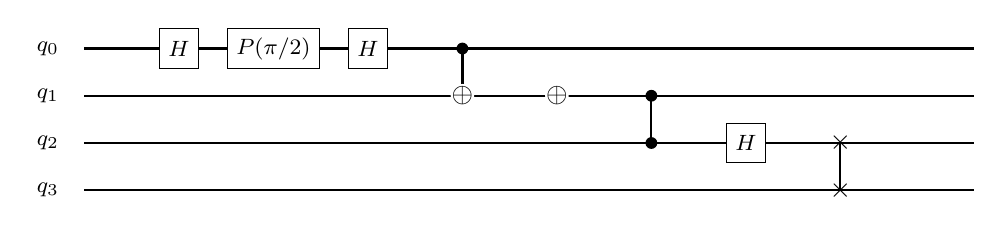
\begin{tikzpicture}[
  wire/.style={thick}]
  \draw[wire] (0,-0.00) -- (11.30,-0.00);
  \node[font=\footnotesize, anchor=east] at (-0.2,-0.00) {$q_{0}$};
  \draw[wire] (0,-0.60) -- (11.30,-0.60);
  \node[font=\footnotesize, anchor=east] at (-0.2,-0.60) {$q_{1}$};
  \draw[wire] (0,-1.20) -- (11.30,-1.20);
  \node[font=\footnotesize, anchor=east] at (-0.2,-1.20) {$q_{2}$};
  \draw[wire] (0,-1.80) -- (11.30,-1.80);
  \node[font=\footnotesize, anchor=east] at (-0.2,-1.80) {$q_{3}$};
  \node[draw, minimum size=0.5cm, fill=white, font=\footnotesize] at (1.20,-0.00) {$H$};
  \node[draw, minimum size=0.5cm, fill=white, font=\footnotesize] at (2.40,-0.00) {$P(\pi/2$)};
  \node[draw, minimum size=0.5cm, fill=white, font=\footnotesize] at (3.60,-0.00) {$H$};
  \draw[thick] (4.80,-0.00) -- (4.80,-0.60);
  \draw[thick] (4.80,-0.60) -- (4.80,-0.00);
  \node[circle, fill=black, minimum size=0.15cm, inner sep=0pt] at (4.80,-0.00) {};
  \node[circle, fill=white, minimum size=3.0mm, inner sep=0pt] at (4.80,-0.60) {};
  \node at (4.80,-0.60) {$\oplus$};
  \node[circle, fill=white, minimum size=3.0mm, inner sep=0pt] at (6.00,-0.60) {};
  \node at (6.00,-0.60) {$\oplus$};
  \draw[thick] (7.20,-1.20) -- (7.20,-0.60);
  \draw[thick] (7.20,-0.60) -- (7.20,-1.20);
  \node[circle, fill=black, minimum size=0.15cm, inner sep=0pt] at (7.20,-1.20) {};
  \node[circle, fill=black, minimum size=0.15cm, inner sep=0pt] at (7.20,-0.60) {};
  \node[draw, minimum size=0.5cm, fill=white, font=\footnotesize] at (8.40,-1.20) {$H$};
  \draw[thick] (9.60,-1.20) -- (9.60,-1.80);
  \draw[thick] (9.60,-1.80) -- (9.60,-1.20);
  \node[font=\normalsize] at (9.60,-1.20) {$\times$};
  \node[font=\normalsize] at (9.60,-1.80) {$\times$};
\end{tikzpicture}
\end{document}
